\documentclass{article}
\usepackage[letterpaper, landscape, margin=0in]{geometry}
\usepackage{showframe}
\usepackage{tikz}
\usepackage[default]{sourcesanspro}
\usepackage[T1]{fontenc}

\pagenumbering{gobble}

\newenvironment{sentencediagram}[5]
    {
        \newgeometry{top=#1in, bottom=#1in, left=#2in, right=#2in}
        \vspace*{\fill}
        \begin{center}
            {
                \fontfamily{cmr}\selectfont
                #3
            }

            \vspace{0.4cm}
            \footnotesize #4, \textit{#5} \\
            \vspace{0.5cm}
            \Large 
    }
    {
        \end{center}
        \vspace*{\fill}
        \clearpage
        \restoregeometry
    }

\definecolor{subjectnoun}{RGB}{106,120,132}
\definecolor{copula}{RGB}{124,139,111}
\definecolor{subjectcomplement}{RGB}{77,47,13}
\definecolor{conjunction}{RGB}{56,84,129}
\definecolor{preposition}{RGB}{64,140,174}
\definecolor{directobject}{RGB}{231,51,143}
\definecolor{adjective}{RGB}{103,81,120}
\definecolor{noun}{RGB}{190,103,93}
\definecolor{predicateverb}{RGB}{176,161,118}
\definecolor{article}{RGB}{62,23,85}
\definecolor{pronoun}{RGB}{0,0,0}
\definecolor{adverb}{RGB}{133,188,114}
\definecolor{modalverb}{RGB}{223,32,88}
\definecolor{infinitiveverb}{RGB}{101,154,148}

\begin{document}
    \begin{sentencediagram}{1.75}{2}{It is a truth universally acknowledged, that a single man in possession of a good fortune, must be in want of a wife.}{Jane Austen}{Pride and Prejudice}
        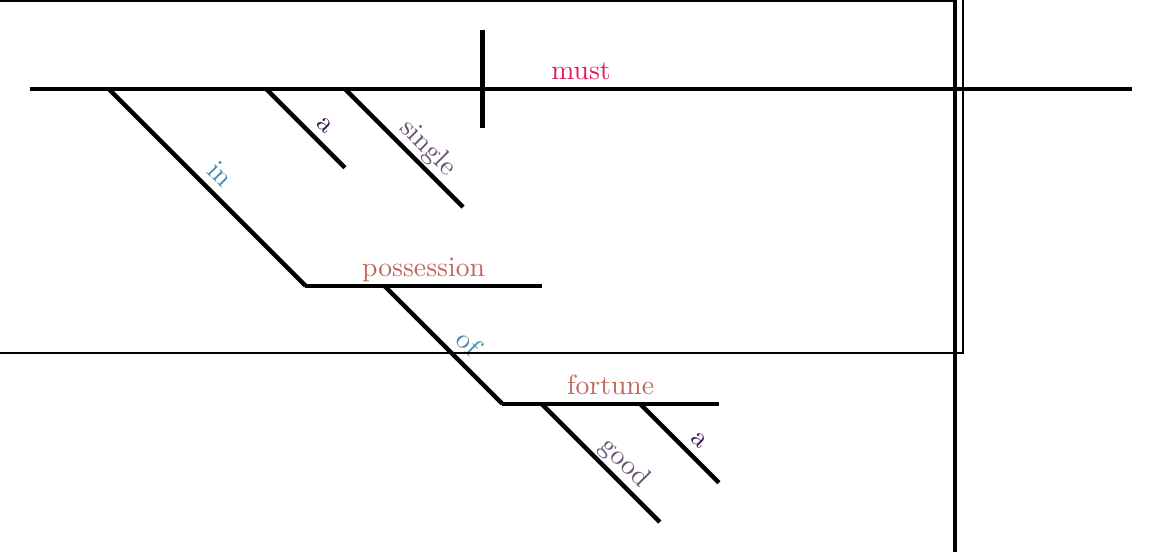
\begin{tikzpicture}
            \tikzstyle{every node} = [above=-0.15cm]
            \draw[ultra thick] (-8, 3) -- (6, 3)
                node[pos=0.5, text=modalverb]{\strut must};
            \draw[ultra thick] (-2.25, 3.75) -- (-2.25, 2.5);

            \draw[ultra thick] (-7, 3) -- (-4.5, 0.5)
                node[sloped, pos=0.5, text=preposition]{\strut in};
            \draw[ultra thick] (-5, 3) -- (-4, 2)
                node[sloped, pos=0.6, text=article]{\strut a};
            \draw[ultra thick]  (-4, 3) -- (-2.5, 1.5)
                node[sloped, pos=0.6, text=adjective]{\strut single};
            \draw[ultra thick] (-4.5, 0.5) -- (-1.5, 0.5)
                node[pos=0.5, text=noun]{\strut possession};

            \draw[ultra thick] (-3.5, 0.5) -- (-2, -1)
                node[sloped, pos=0.6, text=preposition]{\strut of};
            \draw[ultra thick] (-2, -1) -- (0.75, -1)
                node[pos=0.5, text=noun]{\strut fortune};
            \draw[ultra thick] (-1.5, -1) -- (0, -2.5)
                node[sloped, pos=0.6, text=adjective]{\strut good};
            \draw[ultra thick] (-0.25, -1) -- (0.75, -2)
                node[sloped, pos=0.6, text=article]{\strut a};
        \end{tikzpicture}
    \end{sentencediagram}

    \begin{sentencediagram}{2.25}{2.5}{All this happened, more or less.}{Kurt Vonnegut}{Slaughterhouse Five}
        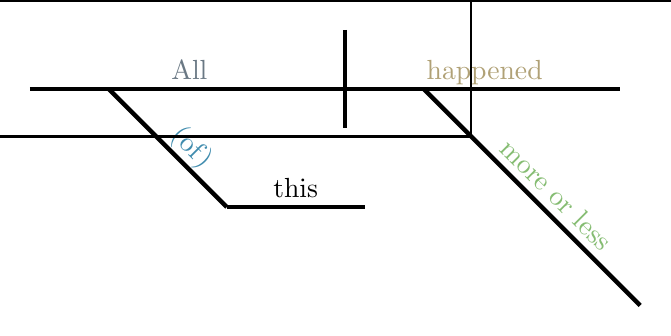
\begin{tikzpicture}
            \tikzstyle{every node} = [above=-0.15cm]
            \draw[ultra thick] (-4.5, 2) -- (3, 2)
                node[pos=0.27, text=subjectnoun]{\strut All}
                node[pos=0.77, text=predicateverb]{\strut happened};
            \draw[ultra thick] (-0.5, 2.75) -- (-0.5, 1.5);

            \draw[ultra thick] (-3.5, 2) -- (-2, 0.5)
                node[sloped, pos=0.6, text=preposition]{\strut (of)};
            \draw[ultra thick] (-2, 0.5) -- (-0.25, 0.5)
                node[pos=0.5, text=pronoun]{\strut this};
            \draw[ultra thick] (0.5, 2) -- (3.25, -0.75)
                node[sloped, pos=0.55, text=adverb]{\strut more or less};
        \end{tikzpicture}
    \end{sentencediagram}

    \begin{sentencediagram}{1.75}{2}{It was a bright cold day in April, and the clocks were striking thirteen.}{George Orwell}{1984}
        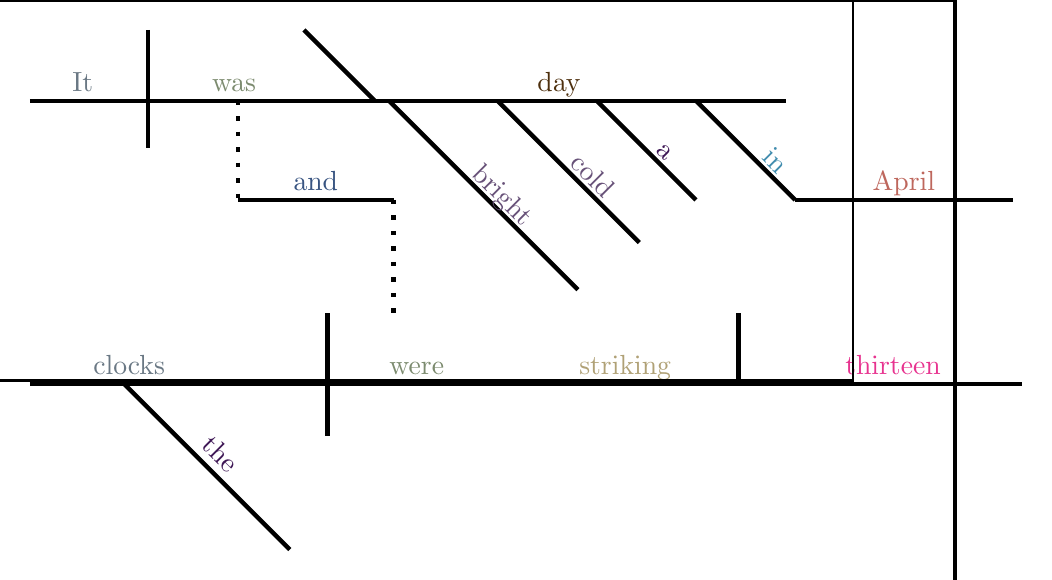
\begin{tikzpicture}[scale=1.2]
            \tikzstyle{every node} = [above=-0.15cm]
            \draw[ultra thick] (-5, 1.75) -- (3, 1.75)
                node[pos=.07, text=subjectnoun]{\strut It}
                node[pos=.27, text=copula]{\strut was}
                node[pos=.7, text=subjectcomplement]{\strut day};
            \draw[ultra thick] (-3.75, 2.5) -- (-3.75, 1.25);
            \draw[ultra thick] (-2.1, 2.5) -- (-1.35, 1.75);
            \draw[ultra thick] (-1.2, 1.75) -- (0.8, -0.25)
                node[above=-0.06cm, sloped, pos=0.55, text=adjective]{\strut bright};
            \draw[ultra thick] (-0.05, 1.75) -- (1.45, 0.25)
                node[above=-0.06cm, sloped, pos=0.6, text=adjective]{\strut cold};
            \draw[ultra thick] (1, 1.75) -- (2.05, 0.7)
                node[above=-0.06cm, sloped, pos=0.6, text=article]{\strut a};
            \draw[ultra thick] (2.05, 1.75) -- (3.1, 0.7)
                node[above=-0.06cm, sloped, pos=0.7, text=preposition]{\strut in};

            \draw[loosely dotted, ultra thick] (-2.8, 1.75) -- (-2.8, 0.7);
            \draw[ultra thick] (-2.8, 0.7) -- (-1.15, 0.7)
                node[pos=.5, text=conjunction]{\strut and};
            \draw[ultra thick] (3.1, 0.7) -- (5.4, 0.7)
                node[pos=.5, text=noun]{\strut April};
            \draw[loosely dotted, ultra thick] (-1.15, 0.7) -- (-1.15, -0.5);

            \draw[ultra thick] (-5, -1.25) -- (5.5, -1.25)
                node[pos=.1, text=subjectnoun]{\strut clocks}
                node[pos=.39, text=copula]{\strut were}
                node[pos=.6, text=predicateverb]{\strut striking}
                node[pos=.87, text=directobject]{\strut thirteen};
            \draw[ultra thick] (-1.85, -0.5) -- (-1.85, -1.8);
            \draw[ultra thick] (2.5, -1.25) -- (2.5, -0.5);
            \draw[ultra thick] (-4, -1.25) -- (-2.25, -3.0)
                node[sloped, pos=.5, text=article]{\strut the};
        \end{tikzpicture}
    \end{sentencediagram}

    \begin{sentencediagram}{2.25}{2.5}{Call me Ishmael.}{Herman Melville}{Moby Dick}
        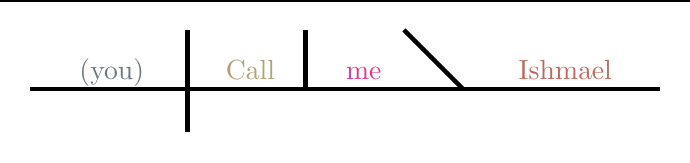
\begin{tikzpicture}
            \tikzstyle{every node} = [above=-0.15cm]
            \draw[ultra thick] (-4, 0) -- (4, 0)
                node[pos=0.13, text=subjectnoun]{\strut (you)}
                node[pos=0.35, text=predicateverb]{\strut Call}
                node[pos=0.53, text=directobject]{\strut me}
                node[pos=0.85, text=noun]{\strut Ishmael};
            \draw[ultra thick] (-2, 0.75) -- (-2, -0.55);
            \draw[ultra thick] (-0.5, 0.75) -- (-0.5, 0);
            \draw[ultra thick] (0.75, 0.75) -- (1.5, 0);
        \end{tikzpicture}
    \end{sentencediagram}

    \begin{sentencediagram}{2.25}{2.5}{It was a pleasure to burn.}{Ray Bradbury}{Fahrenheit 451}
        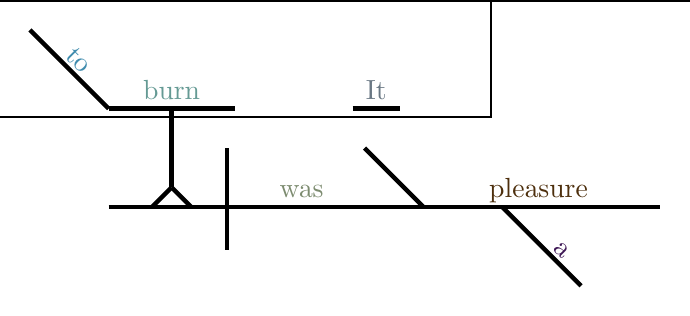
\begin{tikzpicture}
            \tikzstyle{every node} = [above=-0.15cm]
            \draw[ultra thick] (0.1, 1.25) -- (0.7, 1.25)
                node[pos=0.5, text=subjectnoun]{\strut It};

            \draw[ultra thick] (-4, 2.25) -- (-3, 1.25)
                node[above=-0.06cm, sloped, pos=0.5, text=preposition]{\strut to};
            \draw[ultra thick] (-3, 1.25) -- (-1.4, 1.25)
                node[pos=0.5, text=infinitiveverb]{\strut burn};
            \draw[ultra thick] (-2.2, 1.25) -- (-2.2, 0.25);
            \draw[ultra thick] (-2.2, 0.25) -- (-1.95, 0);
            \draw[ultra thick] (-2.2, 0.25) -- (-2.45, 0);

            \draw[ultra thick] (-3, 0) -- (4, 0)
                node[pos=0.35, text=copula]{\strut was}
                node[pos=0.78, text=subjectcomplement]{\strut pleasure};
            \draw[ultra thick] (-1.5, 0.75) -- (-1.5, -0.55);
            \draw[ultra thick] (0.25, 0.75) -- (1, 0);
            \draw[ultra thick] (2, 0) -- (3, -1)
                node[above=-0.06cm, sloped, pos=0.65, text=article]{\strut a};
        \end{tikzpicture}
    \end{sentencediagram}
\end{document}
